% !TEX root = lectures.tex
%!TEX encoding = UTF-8 Unicode
%% !TEX root =  lectures.tex
\documentclass[12pt]{article}
\usepackage{graphicx}
\usepackage[
	pdfencoding=auto,%
	pdftitle={PHY 321, Classical Mechanics I, Lecture Notes},%
	pdfauthor={Scott Pratt},%
	pdfstartview=FitV,%
	colorlinks=true,%
	linkcolor=blue,%
	citecolor=black, %
	urlcolor=blue]{hyperref}
%\usepackage{pdfsync}
\usepackage{amssymb}
\usepackage{amsmath}
\usepackage{bm}
\usepackage{bbold}
\numberwithin{equation}{section} 
\numberwithin{figure}{section} 
\usepackage[small,bf]{caption}

\usepackage{fontspec}
\usepackage{textcomp}
\usepackage{graphicx}
\usepackage{color}
\usepackage{fancyhdr}
\usepackage{bm}

\newcounter{examplecounter}
\setcounter{examplecounter}{0}
\newcommand{\example}{
\stepcounter{examplecounter}{\nopagebreak\noindent\rule{\textwidth}{1pt}\nopagebreak\\ \bf Example \nopagebreak \arabic{section}.\arabic{examplecounter}:\\ \nopagebreak}}

\newcommand{\exampleend}{
\begin{samepage}
\nopagebreak\noindent\rule{\textwidth}{1pt}
\end{samepage}}

%\usepackage[T1]{fontenc}
%\renewcommand*{\sfdefault}{Berenis}
%\renewcommand*{\rmdefault}{Berenis}
%\renewcommand*{\sfdefault}{phv} % helvetica
%\renewcommand*{\sfdefault}{ppl} % palatino
%\renewcommand*{\rmdefault}{ppl}
%\renewcommand*{\sfdefault}{Bookman}
%\renewcommand*{\rmdefault}{Bookman}

\defaultfontfeatures{Scale=MatchLowercase}
%\setmainfont[Mapping=tex-text,SmallCapsFont={CalifornianFB Expert}]{CalifornianFB}
%\setmainfont[Mapping=tex-text]{Minion Pro}
\setmainfont[Mapping=tex-text]{Palatino Bold}
\setmonofont[Mapping=tex-text]{Courier New Bold}
%\setsansfont[Mapping=tex-text]{Myriad Pro}
%\usepackage{xltxtra}
%\setromanfont{Palatino}
\setromanfont{Palatino Bold}


%\pagestyle{empty}
\textwidth 7.0in
\hoffset -0.8in
\textheight 9.4in
\voffset -1in

\pagestyle{fancy}             % page layout
\newcommand{\TheShortTitle}{}
\newcommand{\ShortTitle}[1]{\renewcommand{\TheShortTitle}{#1}}
\fancyhead[LO,RE]{\slshape \TheShortTitle}
\fancyhead[LE,RO]{\slshape \leftmark}

\usepackage{colortbl}
\newcommand{\cc}[1]{\cellcolor{#1}}
\definecolor{lightred}{rgb}{1,0.5,0.6}
\definecolor{lightblue}{rgb}{0.6,0.8,1.0}

\usepackage{comment}
\parskip 4pt
\parindent 0pt

%\newcommand{\bm}{\boldmath}
\boldmath

% for the banner across the tops of pages 2-
\ShortTitle{PHY 831}

\ShortTitle{PHY 321 Lecture Notes}

\section{Gravity and Central Forces}
\bigskip

\subsection{Gravity}

The gravitational potential energy and forces involving two masses $a$ and $b$ are
\begin{eqnarray}
U_{ab}&=&-\frac{Gm_am_b}{|\vec{r}_a-\vec{r}_b|},\\
\nonumber
F_{ba}&=&-\frac{Gm_am_b}{|\vec{r}_a-\vec{r}_b|^2}\hat{r}_{ab},\\
\nonumber
\hat{r}_{ab}&=&\frac{\vec{r}_b-\vec{r}_a}{|\vec{r}_a-\vec{r}_b|}.
\end{eqnarray}
Here $G=6.67\times 10^{-11}$ Nm$^2$/kg$^2$, and $F_{ba}$ is the force on $b$ due to $a$. By inspection, one can see that the force on $b$ due to $a$ and the force on $a$ due to $b$ are equal and opposite. The net potential energy for a large number of masses would be
\begin{equation}
U=\sum_{a<b}U_{ab}=\frac{1}{2}\sum_{a\ne b}U_{ab}.
\end{equation}
Just like electrodynamics, one can define "fields", which for a small additional mass $m$ are the force per mass and the additional potential energy per mass. The {\it gravitational field} related to the force has dimensions of force per mass, or acceleration, and can be labeled $\vec{g}(\vec{r})$. The potential energy per mass has dimensions of energy per mass. This is analogous to the electromagnetic potential, which is the potential energy per charge, and the electric field which is the force per charge.

Because the field $\vec{g}$ obeys the same inverse square law for a point mass as the electric field does for a point charge, the gravitational field also satisfies a version of Gauss's law,
\begin{equation}
\label{eq:GravGauss}
\oint d\vec{A}\cdot\vec{g}=-4\pi GM_{\rm inside}.
\end{equation}
Here, $M_{\rm inside}$ is the net mass inside a closed area.

Gauss's law can be understood by considering a nozzle that sprays paint in all directions uniformly from a point source. Let $B$ be the number of gallons per minute of paint leaving the nozzle. If the nozzle is at the center of a sphere of radius $r$, the paint per square meter per minute that is deposited on some part of the sphere is 
\begin{eqnarray}
F(r)&=&\frac{B}{4\pi r^2}.
\end{eqnarray}
Now, let $F$ also be assigned a direction, so that it becomes a vector pointing along the direction of the flying paint. For any surface that surrounds the nozzle, not necessarily a sphere, one can state that
\begin{eqnarray}
\label{eq:paint}
\oint \vec{dA}\cdot\vec{F}&=&B,
\end{eqnarray}
regardless of the shape of the surface. This follows because the rate at which paint is deposited on the surface should equal the rate at which it leaves the nozzle. The dot product ensures that only the component of $\vec{F}$ into the surface contributes to the deposition of paint. Similarly, if $\vec{F}$ is any radial inverse-square forces, that falls as $B/(4\pi r^2)$, then one can apply Eq. (\ref{eq:paint}). For gravitational fields, $B/(4\pi)$ is replaced by $GM$, and one quickly ``derives'' Gauss's law for gravity, Eq. (\ref{eq:GravGauss}).

\example
Consider Earth to have its mass $M$ uniformly distributed in a sphere of radius $R$. Find the magnitude of the gravitational acceleration as a function of the radius $r$ in terms of the acceleration of gravity at the surface $g(R)$. Assume $r<R$, i.e. you are inside the surface.

{\bf Solution}: Take the ratio of Eq. (\ref{eq:GravGauss}) for two radii, $R$ and $r<R$,
\begin{eqnarray*}
\frac{4\pi r^2 g(r)}{4\pi R^2 g(R)}&=&\frac{4\pi GM_{\rm inside~r}}{4\pi GM_{\rm inside~R}}\\
\nonumber
&=&\frac{r^3}{R^3}\\
\nonumber
g(r)&=&g(R)\frac{r}{R}~.
\end{eqnarray*}

The potential energy per mass is similar conceptually to the voltage, or electric potential energy per charge, that was studied in electromagnetism, if $V\equiv U/m$, $\vec{g}=-\nabla V$.

\exampleend

\subsection{Tidal Forces}

Consider a spherical planet of radius $r$ a distance $D$ from another body of mass $M$. The magnitude of the force due to $M$ on an small object of mass $\delta m$ on surface of the planet can be calculated by performing a Taylor expansion about the center of the spherical planet.
\begin{equation}
F=-\frac{GM\delta m}{D^2}+2\frac{GM\delta m}{D^3}\Delta D+\cdots
\end{equation}
If the $z$ direction points toward the large object, $\Delta D$ can be referred to as $z$. In the accelerating frame of an observer at the center of the planet,
\begin{equation}
\delta m\frac{d^2 z}{dt^2}=F-\delta ma'+{\rm other~forces~acting~on~} \delta m,
\end{equation}
where $a'$ is the acceleration of the observer. Because $\delta ma'$ equals the gravitational force on $\delta m$ if it were located at the planet's center, one can write
\begin{equation}
m\frac{d^2z}{dt^2}=2\frac{GM\delta m}{D^3}z+{\rm other~forces~acting~on~}\delta m.
\end{equation}
Here the other forces could represent the forces acting on $\delta m$ from the spherical planet such as the gravitational force or the contact force with the surface. If $\theta$ is the angle w.r.t. the $z$ axis, the effective force acting on $\delta m$ is
\begin{equation}
F_{\rm eff}\approx 2\frac{GM\delta m}{D^3}r\cos\theta\hat{z}+{\rm other~forces~acting~on~}\delta m.
\end{equation}
This first force is the "tidal" force. It pulls objects outward from the center of the object. If the object were covered with water, it would distort the objects shape so that the shape would be elliptical, stretched out along the axis pointing toward the large mass $M$. The force is always along (either parallel or antiparallel to) the $\hat{z}$ direction.

\begin{samepage}

\example
Consider the Earth to be a sphere of radius $R$ covered with water, with the gravitational acceleration at the surface noted by $g$. Now assume that a distant body provides an additional constant gravitational acceleration $\vec{a}$ pointed along the $z$ axis. Find the distortion of the radius as a function of $\theta$. Ignore planetary rotation and assume $a<<g$.

{\bf Solution}: Because Earth would then accelerate with $a$, the field $a$ would seem invisible in the accelerating frame. A tidal force would only appear if $a$ depended on position, i.e. $\nabla \vec{a}\ne 0$.
\end{samepage}

\example
Now consider that the field is no longer constant, but that instead $a=-kz$ with $|kR|<<g$.

{\bf Solution}: The surface of the planet needs to be at constant potential (if the planet is not accelerating). The force per mass, $-kz$ is like a spring, and the potential per mass is $kz^2/2$. Otherwise water would move to a point of lower potential. Thus, the potential energy for a sample mass $\delta m$ is 
\begin{eqnarray*}
V(R)+\delta m gh(\theta)-\frac{\delta m}{2}kr^2\cos^2\theta={\rm Constant}\\
V(R)+\delta mgh(\theta)-\frac{\delta m}{2}kR^2\cos^2\theta-\delta m kRh(\theta)\cos^2\theta-\frac{\delta m}{2}kh^2(\theta)\cos^2\theta={\rm Constant}.
\end{eqnarray*}
Here, the potential due to the external field is $(1/2)kz^2$ so that $-\nabla U=-kz$. One now needs to solve for $h(\theta)$. Absorbing all the constant terms from both sides of the equation into one constant $C$, and because both $h$ and $kR$ are small, we can through away terms of order $h^2$ or $kRh$. This gives
\begin{eqnarray*}
gh(\theta)-\frac{1}{2}kR^2\cos^2\theta&=&C,\\
h(\theta)&=&\frac{C}{g}+\frac{1}{2g}kR^2\cos^2\theta,\\
h(\theta)&=&\frac{1}{2g}kR^2(\cos^2\theta-1/3).
\end{eqnarray*}
The term with the factor of $1/3$ replaced the constant and was chosen so that the average height of the water would be zero.

\example
The Sun's mass is $27\times 10^6$ the Moon's mass, but the Sun is 390 times further away from Earth as the Sun. What is ratio of the tidal force of the Sun to that of the Moon.

{\bf Solution}: The gravitational force due to an object $M$ a distance $D$ away goes as $M/D^2$, but the tidal force is only the difference of that force over a distance $R$,
\[
F_{\rm tidal}\propto \frac{M}{D^3}R. 
\]
Therefore the ratio of force is
\begin{eqnarray*}
\frac{F_{\rm Sun's~tidal~force}}{F_{\rm Moon's~tidal~force}}
&=&\frac{M_{\rm sun}/D_{\rm sun}^3}{M_{\rm moon}/D_{\rm moon}^3}\\
&=&\frac{27\times 10^6}{390^3}=0.46.
\end{eqnarray*}
The Moon more strongly affects tides than the Sun.

\exampleend

\subsection{Deriving Elliptical Orbits}

Kepler's laws state that a gravitational orbit should be an ellipse with the source of the gravitational field at one focus. Deriving this is surprisingly messy. To do this, we first use angular momentum conservation to transform the equations of motion so that it is in terms of $r$ and $\theta$ instead of $r$ and $t$. The overall strategy is to
\begin{enumerate}\itemsep=0pt
\item Find equations of motion for $r$ and $t$ with no angle ($\theta$) mentioned, i.e. $d^2r/dt^2=\cdots$. Angular momentum conservation will be used, and the equation will involve the angular momentum $L$.
\item Use angular momentum conservation to find an expression for $\dot{\theta}$ in terms of $r$.
\item Use the chain rule to convert the equations of motions for $r$, an expression involving $r,\dot{r}$ and $\ddot{r}$, to one involving $r,dr/d\theta$ and $d^2r/d\theta^2$. This is quitecomplicated because the expressions will also involve a substitution $u=1/r$ so that one finds an expression in terms of $u$ and $\theta$.
\item Once $u(\theta)$ is found, you need to show that this can be converted to the familiar form for an ellipse.
\end{enumerate}

The equations of motion give
\begin{eqnarray}
\label{eq:radialeqofmotion}
\frac{d}{dt}r^2&=&\frac{d}{dt}(x^2+y^2)=2x\dot{x}+2y\dot{y}=2r\dot{r},\\
\nonumber
\dot{r}&=&\frac{x}{r}\dot{x}+\frac{y}{r}\dot{y},\\
\nonumber
\ddot{r}&=&\frac{x}{r}\ddot{x}+\frac{y}{r}\ddot{y}
+\frac{\dot{x}^2+\dot{y}^2}{r}
-\frac{\dot{r}^2}{r}.
\end{eqnarray}
Recognizing that the numerator of the third term is the velocity squared, and that it can be written in polar coordinates, 
\begin{equation}
v^2=\dot{x}^2+\dot{y}^2=\dot{r}^2+r^2\dot{\theta}^2,
\end{equation}
one can write $\ddot{r}$ as
\begin{eqnarray}
\label{eq:radialeqofmotion2}
\ddot{r}&=&\frac{F_x\cos\theta+F_y\sin\theta}{m}+\frac{\dot{r}^2+r^2\dot{\theta}^2}{r}-\frac{\dot{r}^2}{r}\\
\nonumber
&=&\frac{F}{m}+\frac{r^2\dot{\theta}^2}{r}\\
\nonumber
m\ddot{r}&=&F+\frac{L^2}{mr^3}.
\end{eqnarray}
This derivation used the fact that the force was radial, $F=F_r=F_x\cos\theta+F_y\sin\theta$, and that angular momentum is $L=mrv_{\theta}=mr^2\dot{\theta}$. The term $L^2/mr^3=mv^2/r$ behaves like an additional force. Sometimes this is referred to as a centrifugal force, but it is not a force. Instead, it is the consequence of considering the motion in a rotating (and therefore accelerating) frame.

Now, we switch to the particular case of an attractive inverse square force, $F=-\alpha/r^2$, and show that the trajectory, $r(\theta)$, is an ellipse. To do this we transform derivatives w.r.t. time to derivatives w.r.t. $\theta$ using the chain rule combined with angular momentum conservation, $\dot{\theta}=L/mr^2$.
\begin{eqnarray}
\label{eq:rtotheta}
\dot{r}&=&\frac{dr}{d\theta}\dot{\theta}=\frac{dr}{d\theta}\frac{L}{mr^2},\\
\nonumber
\ddot{r}&=&\frac{d^2r}{d\theta^2}\dot{\theta}^2
+\frac{dr}{d\theta}\left(\frac{d}{dr}\frac{L}{mr^2}\right)\dot{r}\\
\nonumber
&=&\frac{d^2r}{d\theta^2}\left(\frac{L}{mr^2}\right)^2
-2\frac{dr}{d\theta}\frac{L}{mr^3}\dot{r}\\
\nonumber
&=&\frac{d^2r}{d\theta^2}\left(\frac{L}{mr^2}\right)^2
-\frac{2}{r}\left(\frac{dr}{d\theta}\right)^2\left(\frac{L}{mr^2}\right)^2
\end{eqnarray}
Equating the two expressions for $\ddot{r}$ in Eq.s (\ref{eq:radialeqofmotion2}) and (\ref{eq:rtotheta}) eliminates all the derivatives w.r.t. time, and provides a differential equation with only derivatives w.r.t. $\theta$,
\begin{equation}
\label{eq:rdotdot}
\frac{d^2r}{d\theta^2}\left(\frac{L}{mr^2}\right)^2
-\frac{2}{r}\left(\frac{dr}{d\theta}\right)^2\left(\frac{L}{mr^2}\right)^2
=\frac{F}{m}+\frac{L^2}{m^2r^3},
\end{equation}
that when solved yields the trajectory, i.e. $r(\theta)$. Up to this point the expressions work for any radial force, not just forces that fall as $1/r^2$.

The trick to simplifying this differential equation for the inverse square problems is to make a substitution, $u\equiv 1/r$, and rewrite the differential equation for $u(\theta)$.
\begin{eqnarray}
r&=&1/u,\\
\nonumber
\frac{dr}{d\theta}&=&-\frac{1}{u^2}\frac{du}{d\theta},\\
\nonumber
\frac{d^2r}{d\theta^2}&=&\frac{2}{u^3}\left(\frac{du}{d\theta}\right)^2-\frac{1}{u^2}\frac{d^2u}{d\theta^2}.
\end{eqnarray}
Plugging these expressions into Eq. (\ref{eq:rdotdot}) gives an expression in terms of $u$, $du/d\theta$, and $d^2u/d\theta^2$. After some tedious algebra,
\begin{equation}
\frac{d^2u}{d\theta^2}=-u-\frac{F m}{L^2u^2}.
\end{equation}
For the attractive inverse square law force, $F=-\alpha u^2$,
\begin{equation}
\frac{d^2u}{d\theta^2}=-u+\frac{m\alpha}{L^2}.
\end{equation}
The solution has two arbitrary constants, $A$ and $\theta_0$,
\begin{eqnarray}
\label{eq:Ctrajectory}
u&=&\frac{m\alpha}{L^2}+A\cos(\theta-\theta_0),\\
\nonumber
r&=&\frac{1}{(m\alpha/L^2)+A\cos(\theta-\theta_0)}.
\end{eqnarray}
The radius will be at a minimum when $\theta=\theta_0$ and at a maximum when $\theta=\theta_0+\pi$. The constant $A$ is related to the eccentricity of the orbit. When $A=0$ the radius is a constant $r=L^2/(m\alpha)$, and the motion is circular. If one solved the expression $mv^2/r=-\alpha/r^2$ for a circular orbit, using the substitution $v=L/(mr)$, one would reproduce the expression $r=L^2/(m\alpha)$.

The form describing the elliptical trajectory in Eq. (\ref{eq:Ctrajectory}) can be identified as an ellipse with one focus being the center of the ellipse by considering the definition of an ellipse as being the points such that the sum of the two distances between the two foci are a constant. Making that distance $2D$, the distance between the two foci as $2a$, and putting one focus at the origin,
\begin{eqnarray}
2D&=&r+\sqrt{(r\cos\theta-2a)^2+r^2\sin^2\theta},\\
\nonumber
4D^2+r^2-4Dr&=&r^2+4a^2-4ar\cos\theta,\\
\nonumber
r&=&\frac{D^2-a^2}{D+a\cos\theta}=\frac{1}{D/(D^2-a^2)-a\cos\theta/(D^2-a^2)}.
\end{eqnarray}
By inspection, this is the same form as Eq. (\ref{eq:Ctrajectory}) with $D/(D^2-a^2)=m\alpha/L^2$ and $a/(D^2-a^2)=A$.

\subsection{Effective or Centrifugal Potential}

The total energy of a particle is 
\begin{eqnarray}
E&=&U(r)+\frac{1}{2}mv_\theta^2+\frac{1}{2}m\dot{r}^2\\
\nonumber
&=&U(r)+\frac{1}{2}mr^2\dot{\theta}^2+\frac{1}{2}m\dot{r}^2\\
\nonumber
&=&U(r)+\frac{L^2}{2mr^2}+\frac{1}{2}m\dot{r}^2.
\end{eqnarray}
The second term then contributes to the energy like an additional repulsive potential. The term is sometimes referred to as the "centrifugal" potential, even though it is actually the kinetic energy of the angular motion. Combined with $U(r)$, it is sometimes referred to as the "effective" potential,
\begin{eqnarray}
U_{\rm eff}(r)&=&U(r)+\frac{L^2}{2mr^2}.
\end{eqnarray}
Note that if one treats the effective potential like a real potential, one would expect to be able to generate an effective force,
\begin{eqnarray}
F_{\rm eff}&=&-\frac{d}{dr}U(r) -\frac{d}{dr}\frac{L^2}{2mr^2}\\
\nonumber
&=&F(r)+\frac{L^2}{mr^3}=F(r)+m\frac{v_\perp^2}{r},
\end{eqnarray}
which is indeed matches the form for $m\ddot{r}$ in Eq. (\ref{eq:radialeqofmotion2}), which included the ``centrifugal'' force.

\example
Consider a particle of mass $m$ in a 2-dimensional harmonic oscillator with potential
\[
U=\frac{1}{2}kr^2=\frac{1}{2}k(x^2+y^2).
\]
If the orbit has angular momentum $L$, find\\
a) the radius and angular velocity of the circular orbit\\
b) the angular frequency of small radial perturbations

{\bf Solution}:\\
a) Consider the effective potential. The radius of a circular orbit is at the minimum of the potential (where the effective force is zero).
\begin{eqnarray*}
U_{\rm eff}&=&\frac{1}{2}kr^2+\frac{L^2}{2mr^2}
\end{eqnarray*}
The effective potential looks like that of a harmonic oscillator for large $r$, but for small $r$, the centrifugal potential repels the particle from the origin. The combination of the two potentials has a minimum for at some radius $r_{\rm min}$.
\begin{eqnarray*}
0&=&kr_{\rm min}-\frac{L^2}{mr_{\rm min}^3},\\
r_{\rm min}&=&\left(\frac{L^2}{mk}\right)^{1/4},\\
\dot{\theta}&=&\frac{L}{mr_{\rm min}^2}=\sqrt{k/m}.
\end{eqnarray*}
For particles at $r_{\rm min}$ with $\dot{r}=0$, the particle does not accelerate and $r$ stays constant, i.e. a circular orbit. The radius of the circular orbit can be adjusted by changing the angular momentum $L$.

b) Now consider small vibrations about $r_{\rm min}$. The effective spring constant is the curvature of the effective potential.
\begin{eqnarray*}
k_{\rm eff}&=&\left.\frac{d^2}{dr^2}U_{\rm eff}(r)\right|_{r=r_{\rm min}}=k+\frac{3L^2}{mr_{\rm min}^4}\\
&=&4k,\\
\omega&=&\sqrt{k_{\rm eff}/m}=2\sqrt{k/m}=2\dot{\theta}.
\end{eqnarray*}
Here, the second step used the result of the last step from part (a). Because the radius oscillates with twice the angular frequency, the orbit has two places where $r$ reaches a minimum in one cycle. This differs from the inverse-square force where there is one minimum in an orbit. One can show that the orbit for the harmonic oscillator is also elliptical, but in this case the center of the potential is at the center of the ellipse, not at one of the foci.

The solution is also simple to write down exactly in Cartesian coordinates. The $x$ and $y$ equations of motion separate,
\begin{eqnarray*}
\ddot{x}&=&-kx,\\
\ddot{y}&=&-ky.
\end{eqnarray*}
So the general solution can be expressed as
\begin{eqnarray*}
x&=&A\cos\omega_0 t+B\sin\omega_0 t,\\
y&=&C\cos\omega_0 t+D\sin\omega_0 t.
\end{eqnarray*}
With some work using double angle formulas, one can calculate
\begin{eqnarray*}
r^2&=&x^2+y^2\\
\nonumber
&=&(A^2+C^2)\cos^2(\omega_0t)+(B^2+D^2)\sin^2\omega_0t+(AB+CD)\cos(\omega_0t)\sin(\omega_0t)\\
\nonumber
&=&\alpha+\beta\cos 2\omega_0 t+\gamma\sin 2\omega_0 t,\\
\alpha&=&\frac{A^2+B^2+C^2+D^2}{2},~~\beta=\frac{A^2-B^2+C^2-D^2}{2},~~\gamma=AB+CD,\\
r^2&=&\alpha+(\beta^2+\gamma^2)^{1/2}\cos(2\omega_0 t-\delta),~~~\delta=\arctan(\gamma/\beta),
\end{eqnarray*}
and see that the radius oscillates with frequency $2\omega_0$. The factor of two comes because the oscillation $x=A\cos\omega_0t$ has two maxima for $x^2$, one at $t=0$ and one a half period later.

\exampleend

\subsection{Stability of Orbits}

The effective force can be extracted from the effective potential, $U_{\rm eff}$. Beginning from the equations of motion, Eq. (\ref{eq:radialeqofmotion}), for $r$,
\begin{eqnarray}
m\ddot{r}&=&F+\frac{L^2}{mr^3}\\
\nonumber
&=&F_{\rm eff}\\
\nonumber
&=&-\partial_rU_{\rm eff},\\
\nonumber
F_{\rm eff}&=&-\partial_r\left[U(r)+(L^2/2mr^2)\right].
\end{eqnarray}
For a circular orbit, the radius must be fixed as a function of time, so one must be at a maximum or a minimum of the effective potential. However, if one is at a maximum of the effective potential the radius will be unstable. For the attractive Coulomb force the effective potential will be dominated by the $-\alpha/r$ term for large $r$ because the centrifugal part falls off more quickly, $\sim 1/r^2$. At low $r$ the centrifugal piece wins and the effective potential is repulsive. Thus, the potential must have a minimum somewhere with negative potential. The circular orbits are then stable to perturbation.

\begin{figure}
\centerline{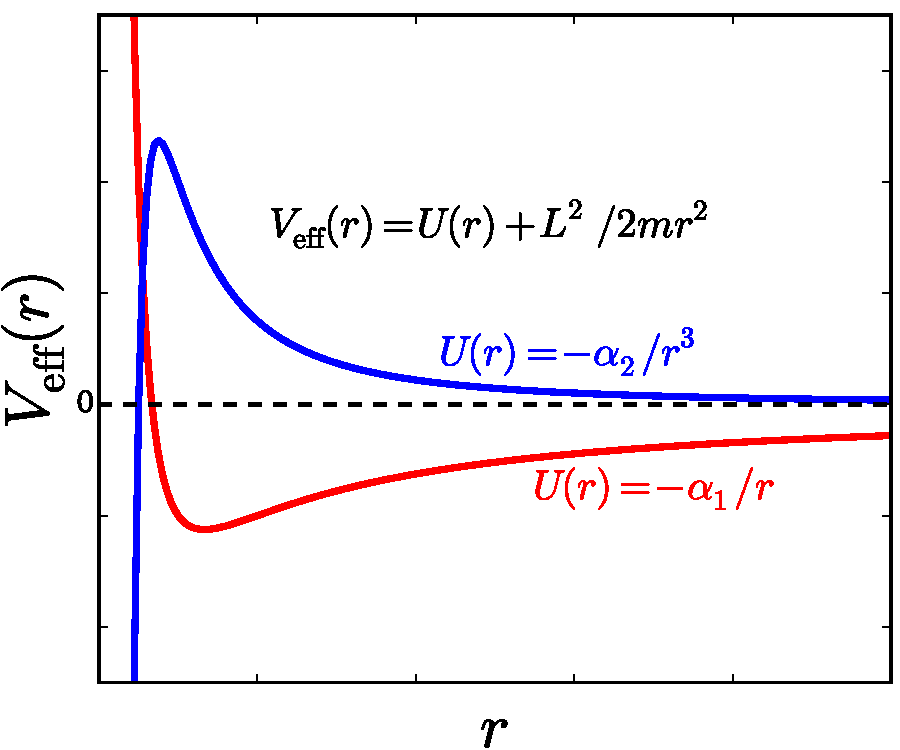
\includegraphics[width=0.45\textwidth]{figs/Veff}}
\caption{\label{fig:Veff}The effective potential is sketched for two cases, a $1/r$ attractive potential and a $1/r^3$ attractive potential. The $1/r$ case has a stable minimum, whereas the circular orbit in the $1/r^3$ case is unstable. 
}
\end{figure}
If one considers a potential that falls as $1/r^3$, the situation is reversed and the point where $\partial_rU$ disappears will be a local maximum rather than a local minimum -- see Fig. \ref{fig:Veff}. The repulsive centrifugal piece dominates at large $r$ and the attractive Coulomb piece wins out at small $r$. The circular orbit is then at a maximum of the effective potential and the orbits are unstable. It is the clear that for potentials that fall as $r^n$, that one must have $n>-2$ for the orbits to be stable.

\example
Consider a potential $U(r)=\beta r$. For a particle of mass $m$ with angular momentum $L$, find the angular frequency of a circular orbit. Then find the angular frequency for small radial perturbations.

{\bf Solution}:\\
For the circular orbit you search for the position $r_{\rm min}$ where the effective potential is minimized,
\begin{eqnarray*}
\partial_r\left\{\beta r+\frac{L^2}{2mr^2}\right\}&=&0,\\
\beta&=&\frac{L^2}{mr_{\rm min}^3},\\
r_{\rm min}&=&\left(\frac{L^2}{\beta m}\right)^{1/3},\\
\dot{\theta}&=&\frac{L}{mr_{\rm min}^2}=\frac{\beta^{2/3}}{(mL)^{1/3}}
\end{eqnarray*}
Now, we can find the angular frequency of small perturbations about the circular orbit. To do this we find the effective spring constant for the effective potential,
\begin{eqnarray*}
k_{\rm eff}&=&\partial_r^2 \left.U_{\rm eff}\right|_{r_{\rm min}}\\
&=&\frac{3L^2}{mr_{\rm min}^4},\\
\omega&=&\sqrt{\frac{k_{\rm eff}}{m}}\\
&=&\frac{\beta^{2/3}}{(mL)^{1/3}}\sqrt{3}.
\end{eqnarray*}
If the two frequencies, $\dot{\theta}$ and $\omega$, differ by an integer factor, the orbit's trajectory will repeat itself each time around. This is the case for the inverse-square force, $\omega=\dot{\theta}$, and for the harmonic oscillator, $\omega=2\dot{\theta}$. In this case, $\omega=\sqrt{3}\dot{\theta}$, and the angles at which the maxima and minima occur change with each orbit.
 
\exampleend

\subsection{Scattering and Cross Sections}

Scattering experiments don't measure entire trajectories. For elastic collisions, they measure the distribution of final scattering angles at best. Most experiments use targets thin enough so that the number of scatterings is typically zero or one. The cross section, $\sigma$, describes the cross-sectional area for particles to scatter with an individual target atom or nucleus. Cross section measurements form the basis for MANY fields of physics. BThe cross section, and the differential cross section, encapsulates everything measurable for a collision where all that is measured is the final state, e.g. the outgoing particle had momentum $\vec{p}_f$. y studying cross sections, one can infer information about the potential interaction between the two particles. Inferring, or constraining, the potential from the cross section is a classic {\it inverse} problem. Collisions are either elastic or inelastic. Elastic collisions are those for which the two bodies are in the same internal state before and after the collision. If the collision excites one of the participants into a higher state, or transforms the particles into different species, or creates additional particles, the collision is inelastic. Here, we consider only elastic collisions.

For Coulomb forces, the cross section is infinite because the range of the Coulomb force is infinite, but for interactions such as the strong interaction in nuclear or particle physics, there is no long-range force and cross-sections are finite. Even for Coulomb forces, the part of the cross section that corresponds to a specific scattering angle, $d\sigma/d\Omega$, which is a function of the scattering angle $\theta_s$ is still finite.

If a particle travels through a thin target, the chance the particle scatters is $P_{\rm scatt}=\sigma dN/dA$, where $dN/dA$ is the number of scattering centers per area the particle encounters. If the density of the target is $\rho$ particles per volume, and if the thickness of the target is $t$, the areal density (number of target scatterers per area) is $dN/dA=\rho t$. Because one wishes to quantify the collisions independently of the target, experimentalists measure scattering probabilities, then divide by the areal density to obtain cross-sections,
\begin{eqnarray}
\sigma=\frac{P_{\rm scatt}}{dN/dA}.
\end{eqnarray}
Instead of merely stating that a particle collided, one can measure the probability the particle scattered by a given angle. The scattering angle $\theta_s$ is defined so that at zero the particle is unscattered and at $\theta_s=\pi$ the particle is scattered directly backward. Scattering angles are often described in the center-of-mass frame, but that is a detail we will neglect for this first discussion, where we will consider the scattering of particles moving classically under the influence of fixed potentials $U(\vec{r})$. Because the distribution of scattering angles can be measured, one expresses the differential cross section,
\begin{equation}
\frac{d^2\sigma}{d\cos\theta_s~d\phi}.
\end{equation}
Usually, the literatures expresses differential cross sections as
\begin{equation}
d\sigma/d\Omega=\frac{d\sigma}{d\cos\theta d\phi}=\frac{1}{2\pi}\frac{d\sigma}{d\cos\theta},
\end{equation}
where the last equivalency is true when the scattering does not depend on the azimuthal angle $\phi$, as is the case for spherically symmetric potentials. 

The differential solid angle $d\Omega$ can be thought of as the area subtended by a measurement, $dA_d$, divided by $r^2$, where $r$ is the distance to the detector,
\begin{eqnarray}
dA_d=r^2 d\Omega.
\end{eqnarray}
With this definition $d\sigma/d\Omega$ is independent of the distance from which one places the detector, or the size of the detector (as long as it is small).

Differential scattering cross sections are calculated by assuming a random distribution of impact parameters $b$. These represent the distance in the $xy$ plane for particles moving in the $z$ direction relative to the scattering center. An impact parameter $b=0$ refers to being aimed directly at the target's center. The impact parameter describes the transverse distance from the $z=0$ axis for the trajectory when it is still far away from the scattering center and has not yet passed it. The differential cross section can be expressed in terms of the impact parameter,
\begin{equation}
d\sigma=2\pi bdb,
\end{equation}
which is the area of a thin ring of radius $b$ and thickness $db$. In classical physics, one can calculate the trajectory given the incoming kinetic energy $E$ and the impact parameter if one knows the mass and potential. From the trajectory, one then finds the scattering angle $\theta_s(b)$. The differential cross section is then
\begin{equation}
\frac{d\sigma}{d\Omega}=\frac{1}{2\pi}\frac{d\sigma}{d\cos\theta_s}=b\frac{db}{d\cos\theta_s}=\frac{b}{(d/db)\cos\theta_s(b)}.
\end{equation}
Typically, one would calculate $\cos\theta_s$ and $(d/db)\cos\theta_s$ as functions of $b$. This is sufficient to plot the differential cross section as a function of $\theta_s$.

The total cross section is 
\begin{equation}
\sigma_{\rm tot}=\int d\Omega\frac{d\sigma}{d\Omega}=2\pi\int d\cos\theta_s~\frac{d\sigma}{d\Omega}. 
\end{equation}
Even if the total cross section is infinite, e.g. Coulomb forces, one can still have a finite differential cross section as we will see later on.

\example
An asteroid of mass $m$ and kinetic energy $E$ approaches a planet of radius $R$ and mass $M$. What is the cross section for the asteroid to impact the planet?

{\bf Solution}:\\
Calculate the maximum impact parameter, $b_{\rm max}$, for which the asteroid will hit the planet. The total cross  section for impact is $\sigma_{\rm impact}=\pi b_{\rm max}^2$. The maximum cross-section can be found with the help of angular momentum conservation. The asteroid's incoming momentum is $p_0=\sqrt{2mE}$ and the angular momentum is $L=p_0b$. If the asteroid just grazes the planet, it is moving with zero radial kinetic energy at impact. Combining energy and angular momentum conservation and having $p_f$ refer to the momentum of the asteroid at a distance $R$,
\begin{eqnarray*}
\frac{p_f^2}{2m}-\frac{GMm}{R}&=&E,\\
p_fR&=&p_0b_{\rm max},
\end{eqnarray*}
allows one to solve for $b_{\rm max}$,
\begin{eqnarray*}
b_{\rm max}&=&R\frac{p_f}{p_0}\\
&=&R\frac{\sqrt{2m(E+GMm/R)}}{\sqrt{2mE}}\\
\sigma_{\rm impact}&=&\pi R^2\frac{E+GMm/R}{E}.
\end{eqnarray*}
\exampleend

\subsection{Center-of-Mass Coordinates}

Thus far, we have considered the trajectory as if the force is centered around a fixed point. For two bodies interacting only with one another, both masses circulate around the center of mass. One might think that solutions would become more complex when both particles move, but we will see here that the problem can be reduced to one with a single body moving according to a fixed force by expressing the trajectories for $\vec{r}_1$ and $\vec{r}_2$ into the center-of-mass coordinate $\vec{R}_{\rm cm}$ and the relative coordinate $\vec{r}$,
\begin{eqnarray}
\vec{R}_{\rm cm}&\equiv&\frac{m_1\vec{r}_1+m_2\vec{r}_2}{m_1+m_2},\\
\nonumber
\vec{r}&\equiv&\vec{r}_1-\vec{r_2}.
\end{eqnarray}
Here, we assume the two particles interact only with one another, so $\vec{F}_{12}=-\vec{F}_{21}$ (where $\vec{F}_{ij}$ is the force on $i$ due to $j$. The equations of motion then become
\begin{eqnarray}
\ddot{\vec{R}}_{\rm cm}&=&\frac{1}{m_1+m_2}\left\{m_1\ddot{\vec{r}}_1+m_2\ddot{\vec{r}}_2\right\}\\
\nonumber
&=&\frac{1}{m_1+m_2}\left\{\vec{F}_{12}+\vec{F}_{21}\right\}=0.\\
\ddot{\vec{r}}&=&\ddot{\vec{r}}_1-\ddot{\vec{r}}_2=\left(\frac{\vec{F}_{12}}{m_1}-\frac{\vec{F}_{21}}{m_2}\right)\\
\nonumber
&=&\left(\frac{1}{m_1}+\frac{1}{m_2}\right)\vec{F}_{12}.
\end{eqnarray}
The first expression simply states that the center of mass coordinate $\vec{R}_{\rm cm}$ moves at a fixed velocity. The second expression can be rewritten in terms of the reduced mass $\mu$.
\begin{eqnarray}
\mu \ddot{\vec{r}}&=&\vec{F}_{12},\\
\frac{1}{\mu}&=&\frac{1}{m_1}+\frac{1}{m_2},~~~~\mu=\frac{m_1m_2}{m_1+m_2}.
\end{eqnarray}
Thus, one can treat the trajectory as a one-body problem where the reduced mass is $\mu$, and a second trivial problem for the center of mass. The reduced mass is especially convenient when one is considering gravitational problems because then
\begin{eqnarray}
\mu \ddot{r}&=&-\frac{Gm_1m_2}{r^2}\hat{r}\\
\nonumber
&=&-\frac{GM\mu}{r^2}\hat{r},~~~M\equiv m_1+m_2.
\end{eqnarray}
For the gravitational problem, the reduced mass then falls out and the trajectory depends only on the total mass $M$.

The kinetic energy and momenta also have analogues in center-of-mass coordinates. The total and relative momenta are
\begin{eqnarray}
\vec{P}&\equiv&\vec{p}_1+\vec{p}_2=M\dot{\vec{R}}_{\rm cm},\\
\nonumber
\vec{q}&\equiv&\mu\dot{\vec{r}}.
\end{eqnarray}
With these definitions, a little algebra shows that the kinetic energy becomes
\begin{eqnarray}
T&=&\frac{1}{2}m_1|\vec{v}_1|^2+\frac{1}{2}m_2|\vec{v}_2|^2\\
\nonumber
&=&\frac{1}{2}M|\dot{\vec{R}}_{\rm cm}|^2
+\frac{1}{2}\mu|\dot{\vec{r}}|^2\\
\nonumber
&=&\frac{P^2}{2M}+\frac{q^2}{2\mu}.
\end{eqnarray}
The standard strategy is to transform into the center of mass frame, then treat the problem as one of a single particle of mass $\mu$ undergoing a force $\vec{F}_{12}$. Scattering angles can also be expressed in this frame, then transformed into the lab frame. In practice, one sees examples in the literature where $d\sigma/d\Omega$ expressed in both the ``center-of-mass'' and in the ``laboratory'' frame. 

\subsection{Rutherford Scattering}

This refers to the calculation of $d\sigma/d\Omega$ due to an inverse square force, $F_{12}=\pm\alpha/r^2$ for repulsive/attractive interaction. Rutherford compared the scattering of $\alpha$ particles ($^4$He nuclei) off of a nucleus and found the scattering angle at which the formula began to fail. This corresponded to the impact parameter for which the trajectories would strike the nucleus. This provided the first measure of the size of the atomic nucleus. At the time, the distribution of the positive charge (the protons) was considered to be just as spread out amongst the atomic volume as the electrons. After Rutherford's experiment, it was clear that the radius of the nucleus tended to be roughly 4 orders of magnitude smaller than that of the atom, which is less than the size of a football relative to Spartan Stadium.

\begin{figure}[!htb]
\centerline{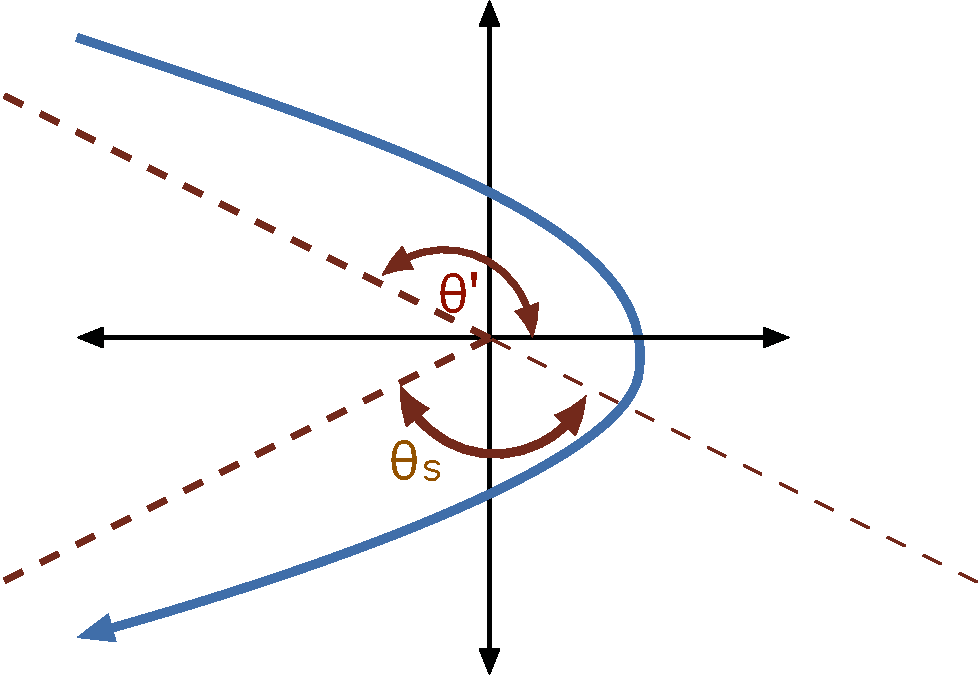
\includegraphics[width=0.6\textwidth]{figs/rutherford}}
\caption{\label{fig:rutherford}
The incoming and outgoing angles of the trajectory are at $\pm\theta'$. They are related to the scattering angle by $2\theta'=\pi+\theta_s$.}
\end{figure}
In order to calculate differential cross section, we must find how the impact parameter is related to the scattering angle. This requires analysis of the trajectory. We consider our previous expression for the trajectory where we derived the elliptic form for the trajectory, Eq. (\ref{eq:Ctrajectory}). For that case we considered an attractive force with the particle's energy being negative, i.e. it was bound. However, the same form will work for positive energy, and repulsive forces can be considered by simple flipping the sign of $\alpha$. For positive energies, the trajectories will be hyperbolas, rather than ellipses, with the asymptotes of the trajectories representing the directions of the incoming and outgoing tracks. Rewriting Eq. (\ref{eq:Ctrajectory}),
\begin{equation}\label{eq:ruthtraj}
r=\frac{1}{\frac{m\alpha}{L^2}+A\cos\theta}.
\end{equation}
Once $A$ is large enough, which will happen when the energy is positive, the denominator will become negative for a range of $\theta$. This is because the scattered particle will never reach certain angles. The asymptotic angles $\theta'$ are those for which the denominator goes to zero,
\begin{equation}
\cos\theta'=-\frac{m\alpha}{AL^2}.
\end{equation}
The trajectory's point of closest approach is at $\theta=0$ and the two angles $\theta'$, which have this value of $\cos\theta'$, are the angles of the incoming and outgoing particles. From Fig. \ref{fig:rutherford}, one can see that the scattering angle $\theta_s$ is given by,
\begin{eqnarray}
\label{eq:sthetover2}
2\theta'-\pi&=&\theta_s,~~~\theta'=\frac{\pi}{2}+\frac{\theta_s}{2},\\
\nonumber
\sin(\theta_s/2)&=&-\cos\theta'\\
\nonumber
&=&\frac{m\alpha}{AL^2}.
\end{eqnarray}
Now that we have $\theta_s$ in terms of $m,\alpha,L$ and $A$, we wish to re-express $L$ and $A$ in terms of the impact parameter $b$ and the energy $E$. This will set us up to calculate the differential cross section, which requires knowing $db/d\theta_s$. It is easy to write the angular momentum as
\begin{equation}
L^2=p_0^2b^2=2mEb^2.
\end{equation}
Finding $A$ is more complicated. To accomplish this we realize that the point of closest approach occurs at $\theta=0$, so from Eq. (\ref{eq:ruthtraj})
\begin{eqnarray}
\label{eq:rminofA}
\frac{1}{r_{\rm min}}&=&\frac{m\alpha}{L^2}+A,\\
\nonumber
A&=&\frac{1}{r_{\rm min}}-\frac{m\alpha}{L^2}.
\end{eqnarray}
Next, $r_{\rm min}$ can be found in terms of the energy because at the point of closest approach the kinetic energy is due purely to the motion perpendicular to $\hat{r}$ and 
\begin{equation}
E=-\frac{\alpha}{r_{\rm min}}+\frac{L^2}{2mr_{\rm min}^2}.
\end{equation}
One can solve the quadratic equation for $1/r_{\rm min}$,
\begin{equation}
\frac{1}{r_{\rm min}}=\frac{m\alpha}{L^2}+\sqrt{(m\alpha/L^2)^2+2mE/L^2}.
\end{equation}
We can plug the expression for $r_{\rm min}$ into the expression for $A$, Eq. (\ref{eq:rminofA}),
\begin{equation}
A=\sqrt{(m\alpha/L^2)^2+2mE/L^2}=\sqrt{(\alpha^2/(4E^2b^4)+1/b^2}
\end{equation}
Finally, we insert the expression for $A$ into that for the scattering angle, Eq. (\ref{eq:sthetover2}),
\begin{eqnarray}
\label{eq:scattangle}
\sin(\theta_s/2)&=&\frac{m\alpha}{AL^2}\\
\nonumber
&=&\frac{a}{\sqrt{a^2+b^2}}, ~~a\equiv \frac{\alpha}{2E}
\end{eqnarray}
The differential cross section can now be found by differentiating the expression for $\theta_s$ with $b$,
\begin{eqnarray}
\label{eq:rutherford}
\frac{1}{2}\cos(\theta_s/2)d\theta_s&=&\frac{ab~db}{(a^2+b^2)^{3/2}}=\frac{bdb}{a^2}\sin^3(\theta_s/2),\\
\nonumber
d\sigma&=&2\pi bdb=\frac{\pi a^2}{\sin^3(\theta_s/2)}\cos(\theta_s/2)d\theta_s\\
\nonumber
&=&\frac{\pi a^2}{2\sin^4(\theta_s/2)}\sin\theta_s d\theta_s\\
\nonumber
\frac{d\sigma}{d\cos\theta_s}&=&\frac{\pi a^2}{2\sin^4(\theta_s/2)},\\
\nonumber
\frac{d\sigma}{d\Omega}&=&\frac{a^2}{4\sin^4(\theta_s/2)}.
\end{eqnarray}
where $a= \alpha/2E$. This the Rutherford formula for the differential cross section. It diverges as $\theta_s\rightarrow 0$ because scatterings with arbitrarily large impact parameters still scatter to arbitrarily small scattering angles. The expression for $d\sigma/d\Omega$ is the same whether the interaction is positive or negative. 

\example
Consider a particle of mass $m$ and charge $z$ with kinetic energy $E$ (Let it be the center-of-mass energy) incident on a heavy nucleus of mass $M$ and charge $Z$ and radius $R$. Find the angle at which the Rutherford scattering formula breaks down.

{\bf Solution}:\\
Let $\alpha=Zze^2/(4\pi\epsilon_0)$. The scattering angle in Eq. (\ref{eq:scattangle}) is 
\[
\sin(\theta_s/2)=\frac{a}{\sqrt{a^2+b^2}}, ~~a\equiv \frac{\alpha}{2E}.
\]
The impact parameter $b$ for which the point of closest approach equals $R$ can be found by using angular momentum conservation,
\begin{eqnarray*}
p_0b&=&b\sqrt{2mE}=Rp_f=R\sqrt{2m(E-\alpha/R)},\\
b&=&R\frac{\sqrt{2m(E-\alpha/R)}}{\sqrt{2mE}}\\
&=&R\sqrt{1-\frac{\alpha}{ER}}.
\end{eqnarray*}
Putting these together
\[
\theta_s=2\sin^{-1}\left\{
\frac{a}{\sqrt{a^2+R^2(1-\alpha/(RE))}}
\right\},~~~a=\frac{\alpha}{2E}.
\]
It was from this departure of the experimentally measured $d\sigma/d\Omega$ from the Rutherford formula that allowed Rutherford to infer the radius of the gold nucleus, $R$.

\exampleend

\subsection{Exercises}

\begin{enumerate}

\item Approximate Earth as a solid sphere of uniform density and radius $R=6360$ km. Suppose you drill a tunnel from the north pole directly to another point on the surface described by a polar angle $\theta$ relative to the north pole. Drop a mass into the hole and let it slide through tunnel without friction. Find the frequency $f$ with which the mass oscillates back and forth. Ignore Earth's rotation. Compare this to the frequency of a low-lying circular orbit.

\item Consider the gravitational field of the moon acting on the Earth.
\begin{enumerate}
\item Calculate the term $k$ in the expansion
\[
g_{\rm moon}=g_0+kz+\cdots,
\]
where $z$ is measured relative to Earth's center and is measured along the axis connecting the Earth and moon. Give your answer in terms of the distance between the moon and the earth, $R_{m}$ and the mass of the moon $M_m$. 
\item Calculate the difference between the height of the oceans at maximum and minimum tides. Express your answer in terms of the quantities above, plus Earth's radius, $R_e$. Then give you answer in meters.
\end{enumerate}

\item Consider an ellipse defined by the sum of the distances from the two foci being $2D$, which expressed in a Cartesian coordinates with the middle of the ellipse being at the origin becomes
\[
\sqrt{(x-a)^2+y^2}+\sqrt{(x+a)^2+y^2}=2D.
\]
Here the two foci are at $(a,0)$ and $(-a,0)$. Show that this form is can be written as
\[
\frac{x^2}{D^2}+\frac{y^2}{D^2-a^2}=1.
\]

\item Consider a particle in an attractive inverse-square potential, $U(r)=-\alpha/r$, where the point of closest approach is $r_{\rm min}$ and the total energy of the particle is $E$. Find the parameter $A$ describing the trajectory in Eq. (\ref{eq:Ctrajectory}). Hint: Use the fact that at $r_{\rm min}$ there is no radial kinetic energy and $E=-\alpha/r_{\rm min}+L^2/2mr_{\rm min}^2$.

\item Consider the effective potential for an attractive inverse-square-law force, $F=-\alpha/r^2$. Consider a particle of mass $m$ with angular momentum $L$.
\begin{enumerate}
\item Find the radius of a circular orbit by solving for the position of the minimum of the effective potential. 
\item What is the angular frequency, $\dot{\theta}$, of the orbit? Solve this by setting $F=m\dot{\theta}^2r$.
\item Find the effective spring constant for the particle at the minimum.
\item What is the angular frequency for small vibrations about the minimum? How does this compare with the answer to (b)?
\end{enumerate}

\item Consider a particle of mass $m$ moving in a potential
\[
U=\alpha\ln(r/a).
\]
\begin{enumerate}
\item If the particle is moving in a circular orbit of radius $R$, find the angular frequency $\dot{\theta}$. Solve this by setting $F=-m\dot{\theta}^2r$ (force and acceleration point inward).
\item Express the angular momentum $L$ in terms of $\alpha$, $m$ and $R$. Also express $R$ in terms of $L$, $\alpha$ and $m$.
\item Sketch the effective radial potential, $V_{\rm eff}(r)$, for a particle with angular momentum $L$. (No longer necessarily moving in a circular orbit.)
\item Find the position of the minimum of $V_{\rm eff}$ in terms of $L$, $\alpha$ and $m$, then compare to the result of (b).
\item What is the effective spring constant for a particle at the minimum of $V_{\rm eff}$? Express your answer in terms of $L$, $m$ and $\alpha$. 
\item What is the angular frequency, $\omega$, for small oscillations of $r$ about the $R_{\rm min}$?  Express your answer in terms of $\dot{\theta}$ from part (a).
\end{enumerate}

\item Consider a particle of mass $m$ in an attractive potential, $U(r)=-\alpha/r$, with angular momentum $L$ with just the right energy so that
\[
A=m\alpha/L^2
\]
where $A$ comes from the expression
\[
r=\frac{1}{(m\alpha/L^2)+A\cos\theta}.
\]
The trajectory can then be rewritten as
\[
r=\frac{2r_0}{1+\cos\theta},~~~r_0=\frac{L^2}{2m\alpha}.
\]
\begin{enumerate}
\item Show that for this case the total energy $E$ approaches zero.
\item Write this trajectory in a more recognizable parabolic form,
\[
x=x_0-\frac{y^2}{R}.
\]
I.e., express $x_0$ and $R$ in terms of $r_0$.
\item Explain how a particle with zero energy can have its trajectory not go through the origin.
\item What is the scattering angle for this trajectory?
\end{enumerate}

\item Show that if one transforms to a reference frame where the total momentum is zero, $\vec{p}_1=-\vec{p}_2$, that the relative momentum $\vec{q}$ corresponds to either $\vec{p}_1$ or $-\vec{p}_2$. This means that in this frame the magnitude of $\vec{q}$ is one half the magnitude of $\vec{p}_1-\vec{p}_2$.

\item Given the center of mass coordinates $\vec{R}$ and $\vec{r}$ for particles of mass $m_1$ and $m_2$, find the coordinates $\vec{r}_1$ and $\vec{r}_2$ in terms of the masses, $\vec{R}$ and $\vec{r}$.

\item Consider two particles of identical mass scattering at an angle $\theta_{\rm cm}$ in the center of mass.
\begin{enumerate}
\item In a frame where one is the target (initially at rest) and one is the projectile, find the scattering angle in the lab frame, $\theta$, in terms of $\theta_{\rm cm}$.
\item Express $d\sigma/d\cos\theta$ in terms of $d\sigma/d\cos\theta_{\rm cm}$. I.e., find the Jacobian, $d\cos\theta_{\rm cm}/d\cos\theta$.
\end{enumerate}

\item Assume you are scattering alpha particles (He-4 nuclei $Z=2, A=4$) off of a gold target ($Z=79, A=197$). If the radius of the nucleus is $7.5\times 10^{-15}$ meters, and if the energy of the beam is 38 MeV,
\begin{enumerate}
\item What is the total cross section for having a nuclear collision? Give the answer in millibarns, 1 mb$=10^{-31}$ m$^2$.
\item Find the scattering angle (in degrees) at which the Rutherford differential cross section formula breaks down?

\end{enumerate}
\end{enumerate}
%\end{document}
